\chapter{Experimental Results} \label{chap:experimental-results}
In this chapter we present the experimental setup on which the proposed architecture has been developed, implemented and tested.
First we will present the master and slave robots,  then the general architecture is explained and finally we discuss on the impact that the limits of such setup have on the implementation.

\section{Manipulators}
This bilateral teleoperation setup is based upon two of the manipulators available in the Altair laboratory of the University of Verona.
The master console is a Sensable Phantom Omni (recently rebranded as 3D-System Touch).
The slave device is a Barret WAM in the 7-DoF configuration.




\begin{table}[htbp]
	\resizebox{\textwidth}{!}{%
		\begin{tabular}{|c|c|c|c|c|c|c|c|c|c|} 
			\hline
			Setup 			 	& Odom VOVD & Track Pipe & Decompression & Frame Elaboration & Feature Extraction & Publish Pose & FPS Track & FPS Feature Extraction & FPS Supported \\ 
			\hline
			orb(j1)     		&	-  		& 43,41 	 & 13,08 		 & 49,21 			 & 43,62 			  & 0,02		 & 23,04	 & 20,32				  & 20,32 		  \\
			\rowcolor{Gray}
			vovd(j1)       	 	& 1,70 		& -     	 & -    		 & -     			 & -    			  & -   		 & -     	 & -    				  & -     		  \\
			(orb;vovd)(j1)      & 2,58 		& 73,49 	 & 18,69 		 & 62,70 			 & 54,76 			  & 0,17		 & 13,61 	 & 15,95				  & 13,61 		  \\
			\rowcolor{Gray}
			(orb(j1);vovd(j2))  & 1,60 		& 49,81 	 & 13,53 		 & 49,25 			 & 43,01			  & 0,08 		 & 20,08	 & 20,30 				  & 20,08		  \\
			\hline
	\end{tabular}}
	\caption{Performance Measurement: camera 10 Hz \label{tab:Performance-Measurement-10hz}}
\end{table}


\begin{table}[htbp]
	\resizebox{\textwidth}{!}{%
		\begin{tabular}{|c|c|c|c|c|c|c|c|c|c|} 
			\hline
			Setup 			 	& Odom VOVD & Track Pipe & Decompression & Frame Elaboration & Feature Extraction & Publish Pose & FPS Track & FPS Feature Extraction & FPS Supported \\ 
			\hline
			orb(j1)     		&   -  & 54,82 & 14,47 & 49,40 & 44,35 & 0,02 & 18,24 & 20,24 & 18,24 \\
			\rowcolor{Gray}
			vovd(j1)       	 	& 1,70 & -     & -     & -     & -     & -    & -     & -     & -     \\
			(orb;vovd)(j1)      & 2,85 & 93,15 & 23,96 & 67,99 & 60,41 & 0,21 & 10,74 & 14,71 & 10,74 \\
			\rowcolor{Gray}
			(orb(j1);vovd(j2))  & 1,60 & 56,20 & 14,00 & 49,32 & 43,95 & 0,09 & 17,79 & 20,27 & 17,79 \\
			\hline
	\end{tabular}}
	\caption{Performance Measurement: camera 20 Hz \label{tab:Performance-Measurement-20hz}}
\end{table}




\begin{table}[htbp]
	\resizebox{\textwidth}{!}{%
		\begin{tabular}{|c|c|c|c|c|c|c|c|c|c|} 
			\hline
			Setup 			 	& Odom VOVD & Track Pipe & Decompression & Frame Elaboration & Feature Extraction & Publish Pose & FPS Track & FPS Feature Extraction & FPS Supported \\ 
			\hline
			orb(j1)     		& -    & 42,98 & 35,43 & 82,05 & 55,70 & 0,01 & 23,27 & 12,19 & 12,19 \\
			\rowcolor{Gray}
			vovd(j1)       	 	& 1,23 & -     & -     & -     & -     & -    & -     & -     & -     \\
			(orb;vovd)(j1)      & 1,40 & 66,13 & 30,09 & 69,10 & 63,75 & 0,16 & 15,12 & 14,47 & 14,47 \\
			\rowcolor{Gray}
			(orb(j1);vovd(j2))  & 1,24 & 46,62 & 30,10 & 74,16 & 67,80 & 0,52 & 21,45 & 13,48 & 13,48 \\
			\hline
	\end{tabular}}
	\caption{kubeedge - Performance Measurement: camera 10 Hz \label{tab:kubeedge-Performance-Measurement-10hz}}
\end{table}


\begin{table}[htbp]
	\resizebox{\textwidth}{!}{%
		\begin{tabular}{|c|c|c|c|c|c|c|c|c|c|} 
			\hline
			Setup 			 	& Odom VOVD & Track Pipe & Decompression & Frame Elaboration & Feature Extraction & Publish Pose & FPS Track & FPS Feature Extraction & FPS Supported \\ 
			\hline
			orb(j1)     		& -    & 38,56 & 32,65 & 80,31 & 55,48 & 0,01 & 25,93 & 12,45 & 12,45 \\
			\rowcolor{Gray}
			vovd(j1)       	 	& 1,21 & -     & -     & -     & -     & -    & -     & -     & -     \\
			(orb;vovd)(j1)      & 1,43 & 74,00 & 28,48 & 68,90 & 63,11 & 0,15 & 13,51 & 14,51 & 13,51 \\
			\rowcolor{Gray}
			(orb(j1);vovd(j2))  & 1,26 & 51,40 & 27,33 & 66,86 & 62,50 & 0,23 & 19,46 & 14,96 & 14,96 \\
			\hline
	\end{tabular}}
	\caption{Kubeedge - Performance Measurement: camera 20 Hz \label{tab:kubeedge-Performance-Measurement-20hz}}
\end{table}










\subsection{Phantom Omni}
The Phantom Omni is a commercial, portable haptic device with six Degrees of Freedom (DoF) with the three translational degrees of freedom actuated, developed by Sensable Technologies. It is based on a serial architecture, which means that the handle is connected to the housing by a single serial chain.
The device evolved from research done by Thomas Massie and Dr. Kenneth Salisbury at MIT.

The workspace of the Phantom Omni is 16cm $\times$ 12cm $\times$ 7 cm (W $\times$ H $\times$ D) and can provide a peak force feedback up to 3.3 N. Thanks to its six DoFs and a nominal position resolution of around 0.055 mm the device is used in various professional environments. The Phantom Omni is currently sold by 3D-System under the product name Touch.
The models available in the lab are the firewire  and USB ones, both lacks of driver support for modern Linux distributions. Thus a Windows machine is a mandatory requirement to adopt the Phantom Omni in this setup.

The device ships with its SDK, OpenHaptics, designed for a simple control of the device.
It provides two abstraction levels: namely HU and HD. The former it's oriented to provides haptic feedbacks from a virtual graphics scenario, the latter is close tight to the hardware and provides the Phantom's status information like stylus pose, stylus velocity and pressed buttons.\\
The available data vary upon the availability of actuated DoF on device in use: for the Omni model the API does not provide either angular velocity or the evaluated geometric Jacobian.
The pose frame of reference, which is not clearly addressed in the documentation, has been empirically found in the middle of the Cartesian workspace.
Finally, this is another unclear point from the available documentation, the pose provided by the HD API refers not to the stylus tip, but to the middle point of the gimbal.
These are useful information when dealing with the virtual model of the device.
A custom version of the urdf model \cite{Omni_urdf} enables the correct visualization of the pose from HD API into the RVIZ visualizer.

\begin{figure}
	\subfloat[The Phantom Omni]{
		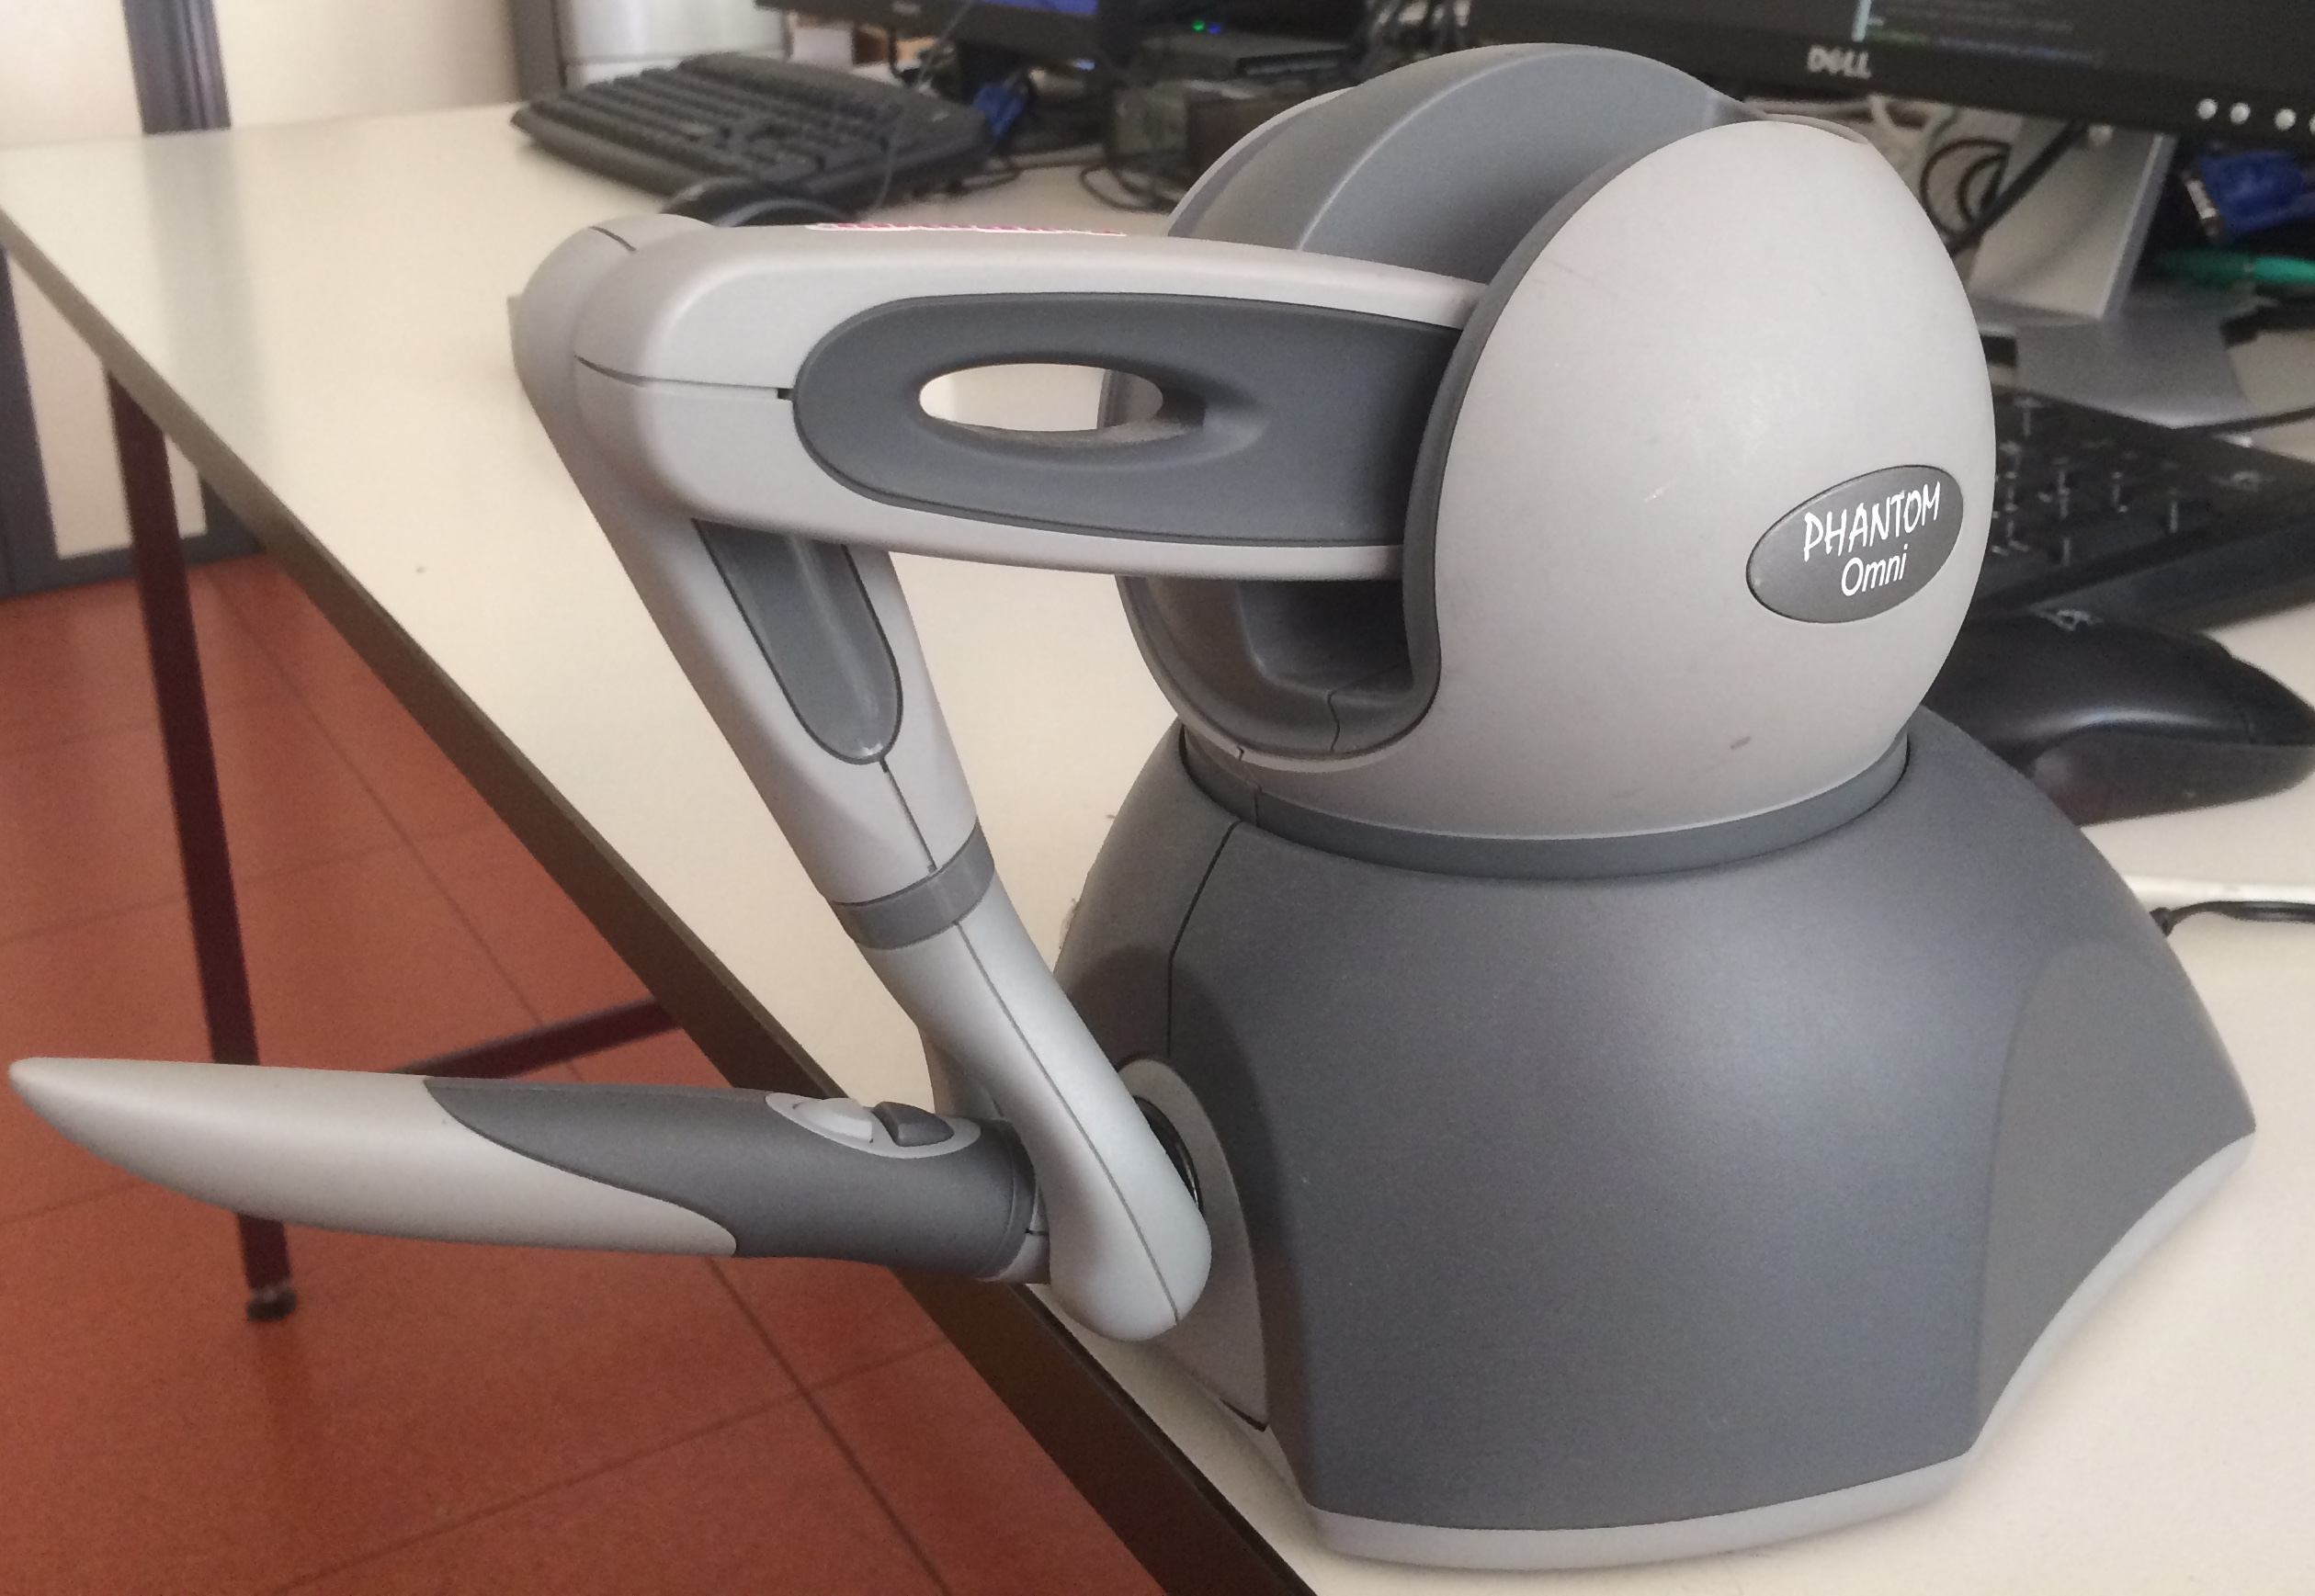
\includegraphics[width=\linewidth/2]{images/omni.jpeg}
		\label{fig:omni}}
	\subfloat[The WAM available in Altair Laboratory while performin a puncturing test]{	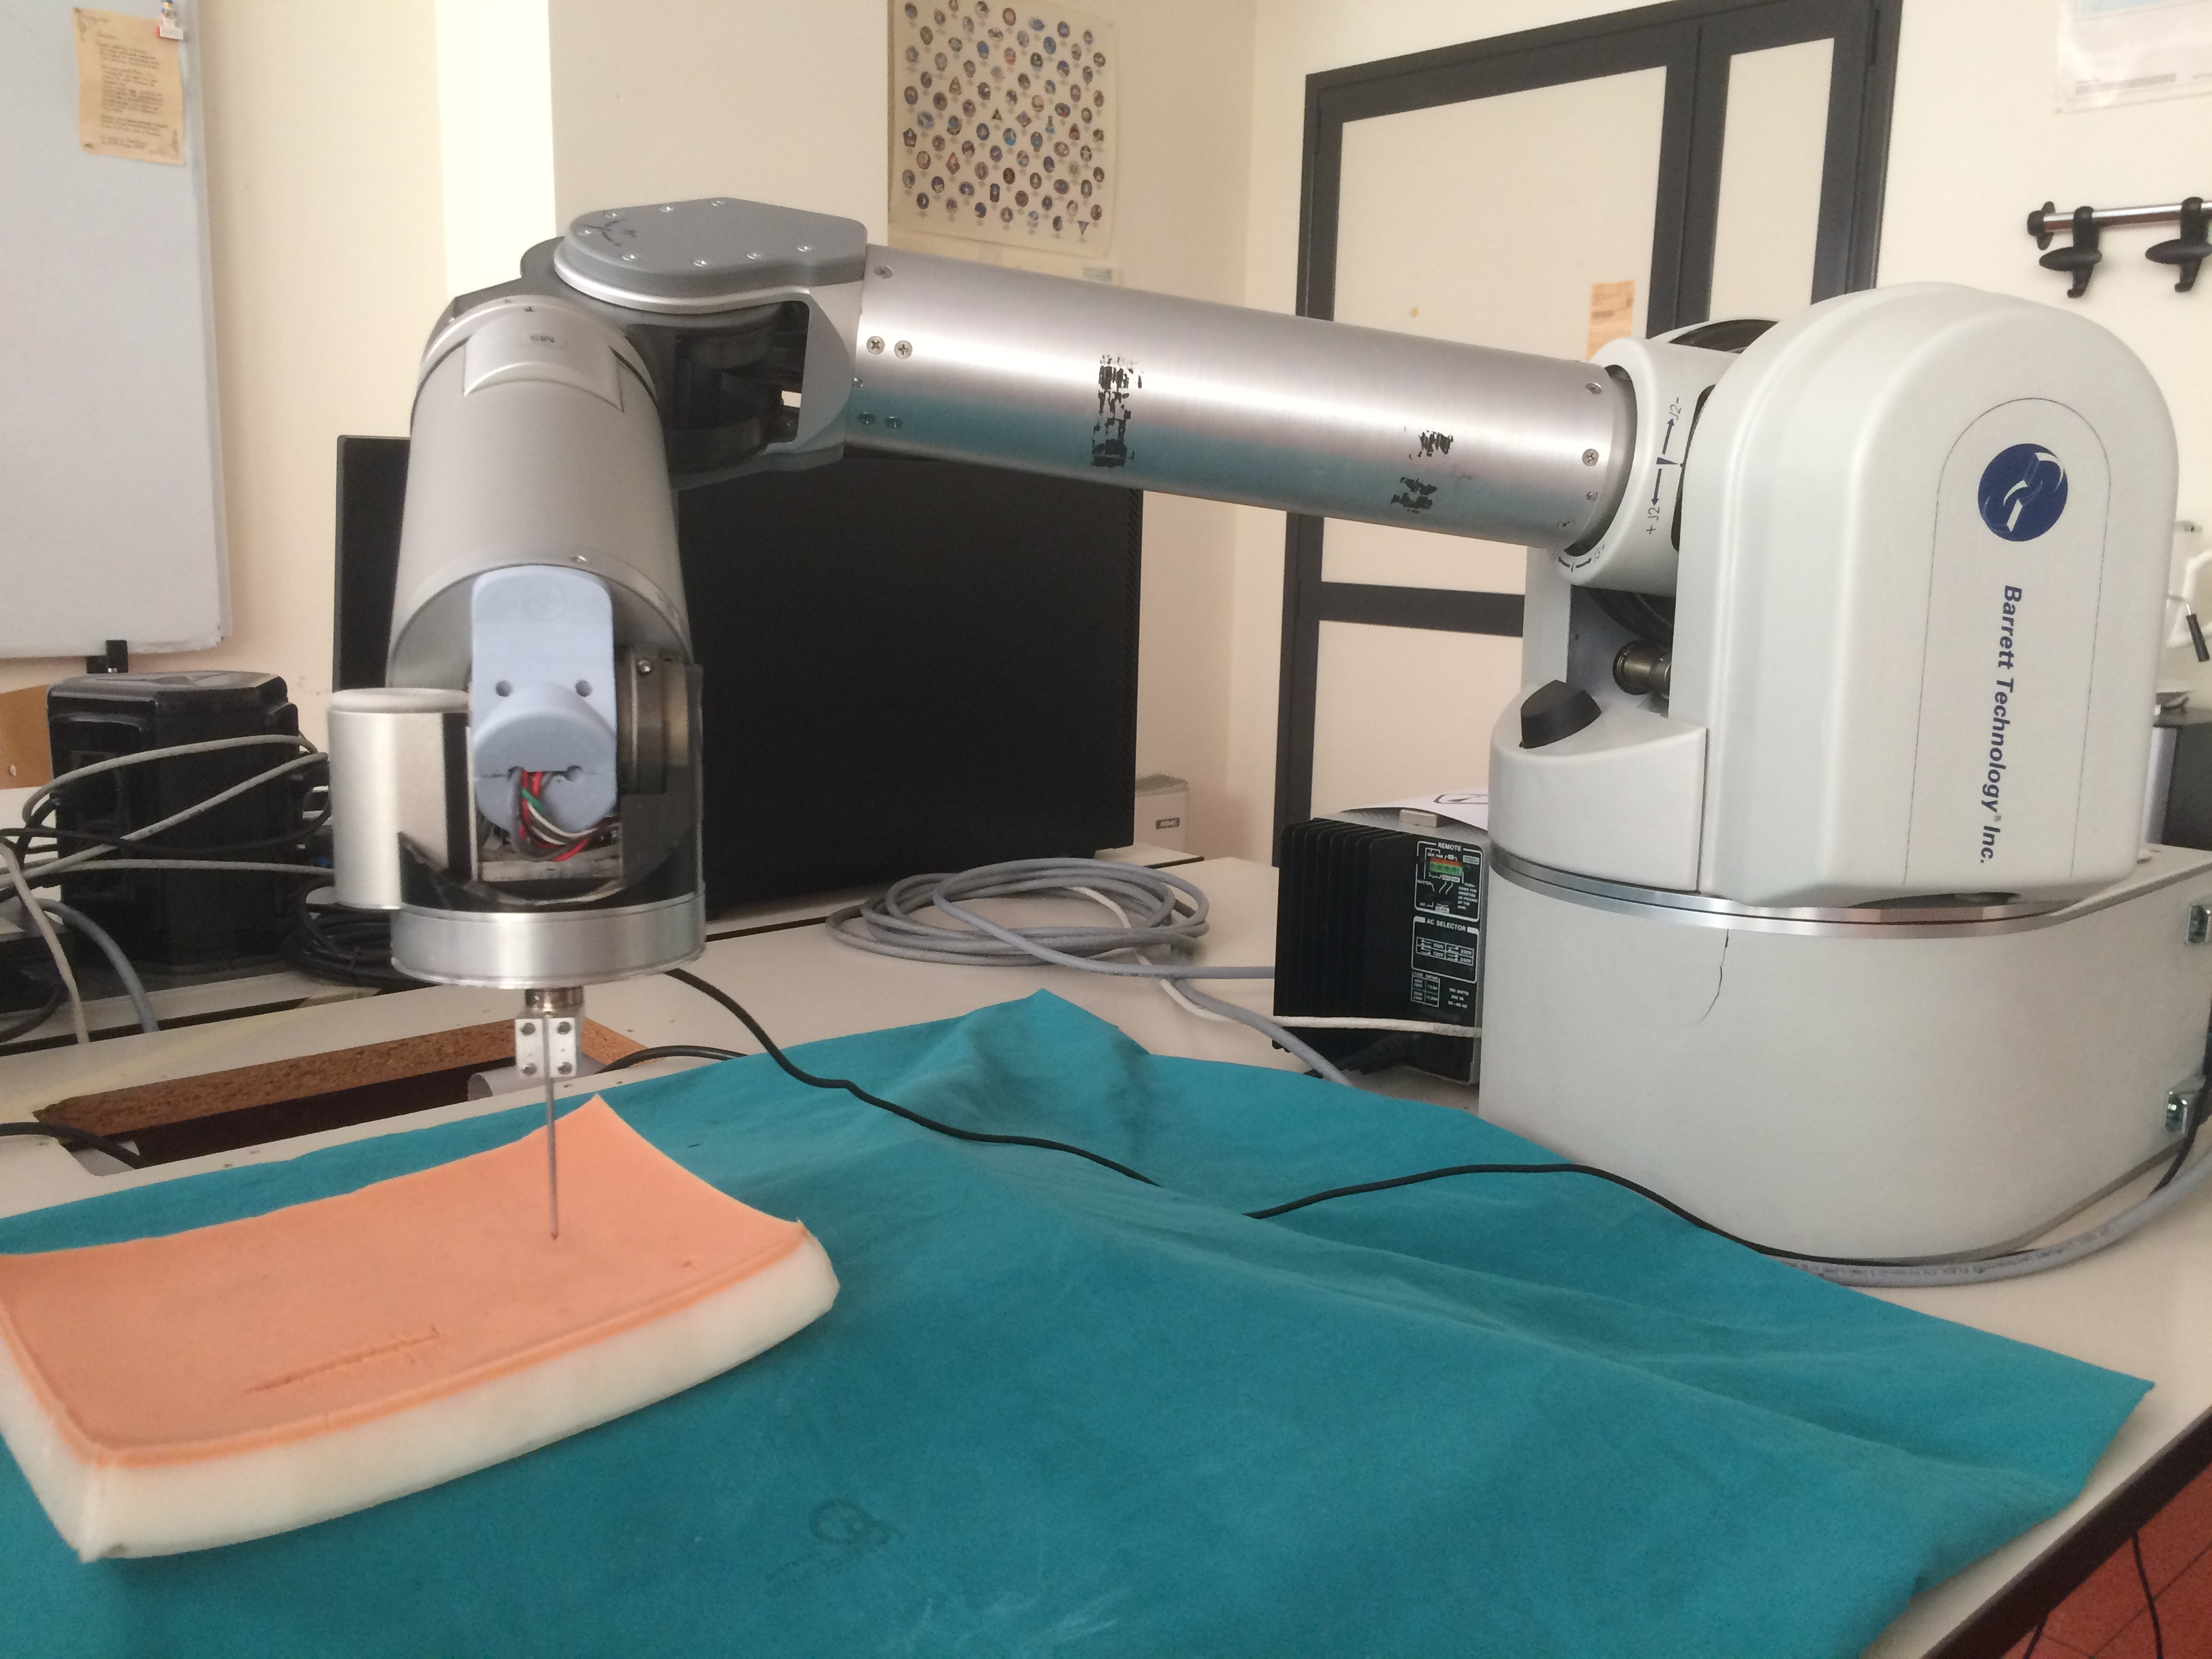
\includegraphics[width=\linewidth/2]{images/WAM_puncture.jpeg}
	\label{fig:WAM_puncture}}
\caption[The WAM and Phantom Omni]{The two manipulators}
\label{fig:EE}
\end{figure}

\subsection{WAM}
The robotic arm used in this setup as slave robot is called WAM, from Barrett Techonology.
The WAM is a manipulator available in two main configurations, 4 and 7-DoF, both with human-like kinematics.
The manipulator available at the Altair laboratory has the seven degrees of freedom configuration, which offers better adaptability and dexterity and is shown in \figurename{ \ref{fig:WAM_puncture}}.\\
The uniqueness of the WAM arm lies in its backdriven cable drives, similar to human tendons. This kind of design concentrates the weight at its base and makes the whole arm light enough to have little brake time together  with high  acceleration and flexibility. Moreover, its lightness translates into power saving.
\tablename{ \ref{WAM_DH}} its the \textit{Denavit-Hartenberg} parameters of the Barrett Wam's arm.
\begin{table} 
\centering
\begin{tabular}{>{\itshape}lcccc}
	\toprule
	&$\theta$ & d & a & $\alpha$\\
	\midrule
	\multirow{7}*{Robot}&$\theta_{1}$  & 0 & 0 & $-\pi/2$ \\
	&$\theta_{2}$  & 0	& 0 & $\pi/2$ \\
	&$\theta_{3}$  & 0,55 & 0,045 & $-\pi/2$ \\
	&$\theta_{4}$  & 0 & -0,045 & $\pi/2$\\
	&$\theta_{5}$  & 0,3 & 0 & $-\pi/2$ \\
	&$\theta_{6}$  & 0 & 0&$\pi/2$ \\
	&$\theta_{7}$  & 0,06& 0 & 0 \\
	\midrule
	End-Effector&$-0,16\pi$ & 0,085 & 0,08 & 0\\
	\bottomrule
\end{tabular}
\caption[WAM D-H parameters]{D-H parameters of the WAM manipulator with needle holder as end-effector}
\label{WAM_DH}
\end{table}

For the purpose of this work, a needle with its holder has been mounted at the end effector.
The assembly includes a force sensor, the ATI Nano 17, that provides the external interaction forces in the Position - Force teleoperation schema.
The whole assembly, from its base to the needle's tip, could be seen as a unique static transformation that could be added at the end of the WAM's kinematic chain (the last line in \tablename{ \ref{WAM_DH}}).
\figurename{ \ref{fig:EE2}} shows the WAM end-effector.
\begin{figure}
	\subfloat[Schematics of the whole needle holder assembly]{	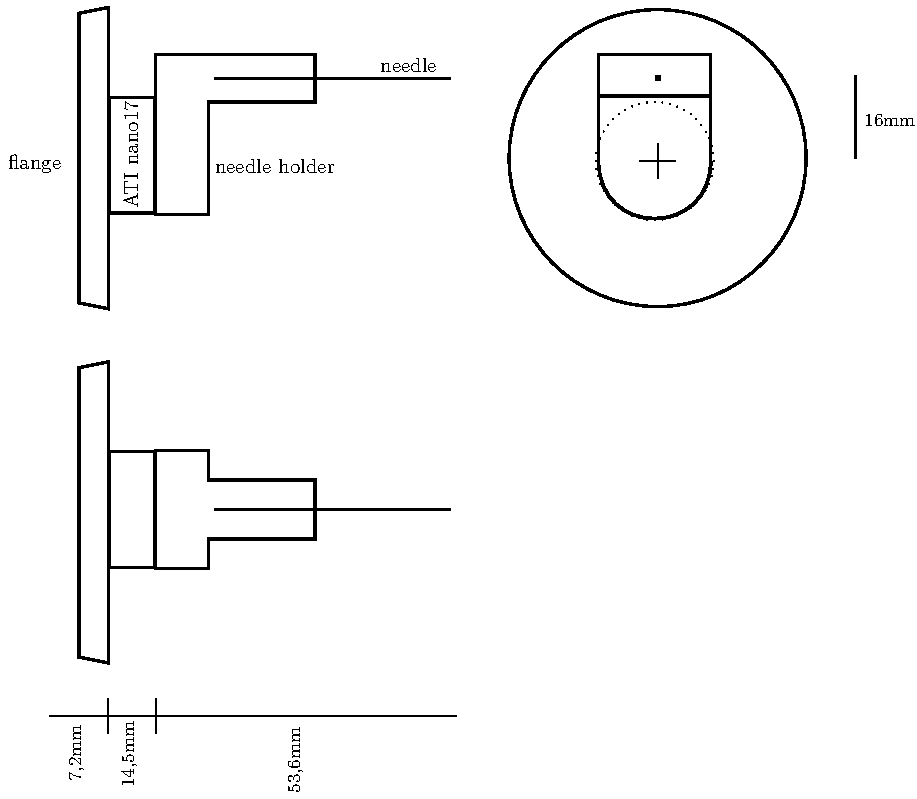
\includegraphics[width=\linewidth/2]{schemas/Needle_holder_assembly.pdf}
		\label{sch:Needle_holder_assembly}}
	\subfloat[The end-effector]{
	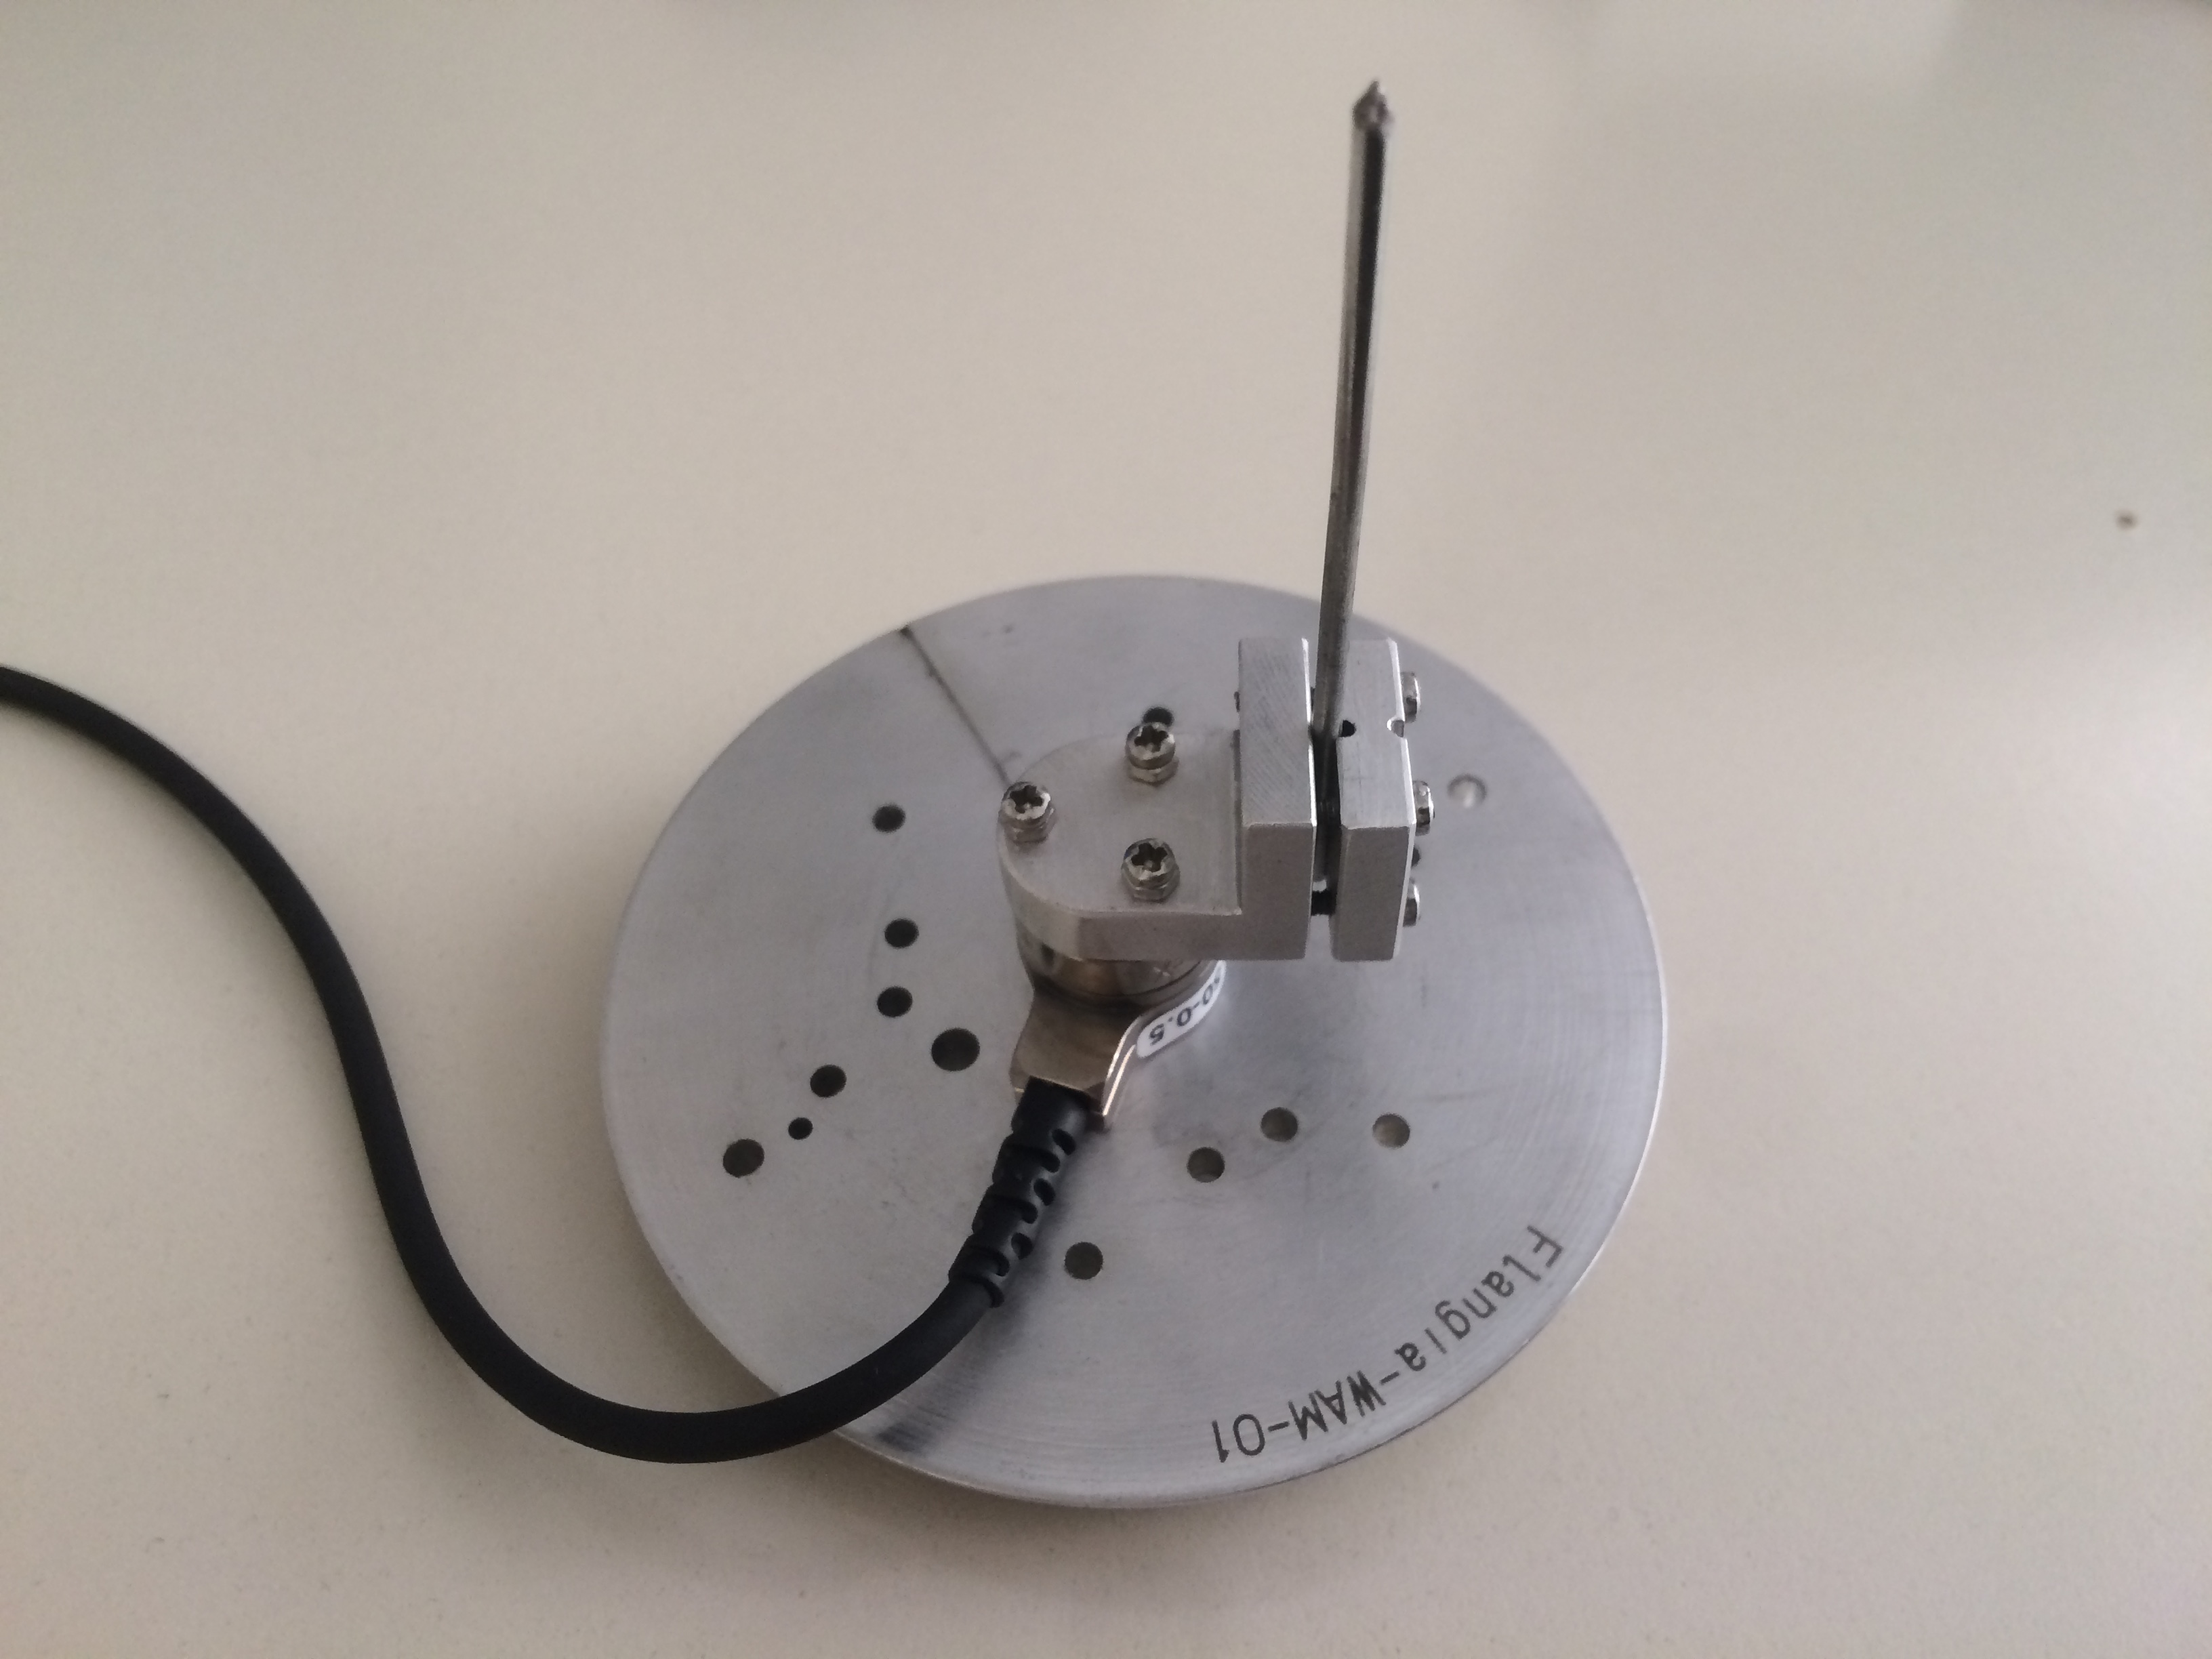
\includegraphics[width=\linewidth/2]{images/needle_holder.jpeg}
	\label{fig:Needle_holder_assembly}}
	\caption[The needle holder assembly]{The needle holder assembly}
	\label{fig:EE2}
\end{figure}

In this thesis we are focusing on the feasibility of the teleoperation architecture thus we are not interest on dealing with needle bending. Because of that, we applied to the needle holder a nail that represent an acceptable trade-off for our intent.
However, with a different needle holder shown in \figurename{ \ref{fig:New_holder}} that has been designed in the meanwhile, in future we will be able to evaluate the system with a real crioablation needle.
\begin{figure}
	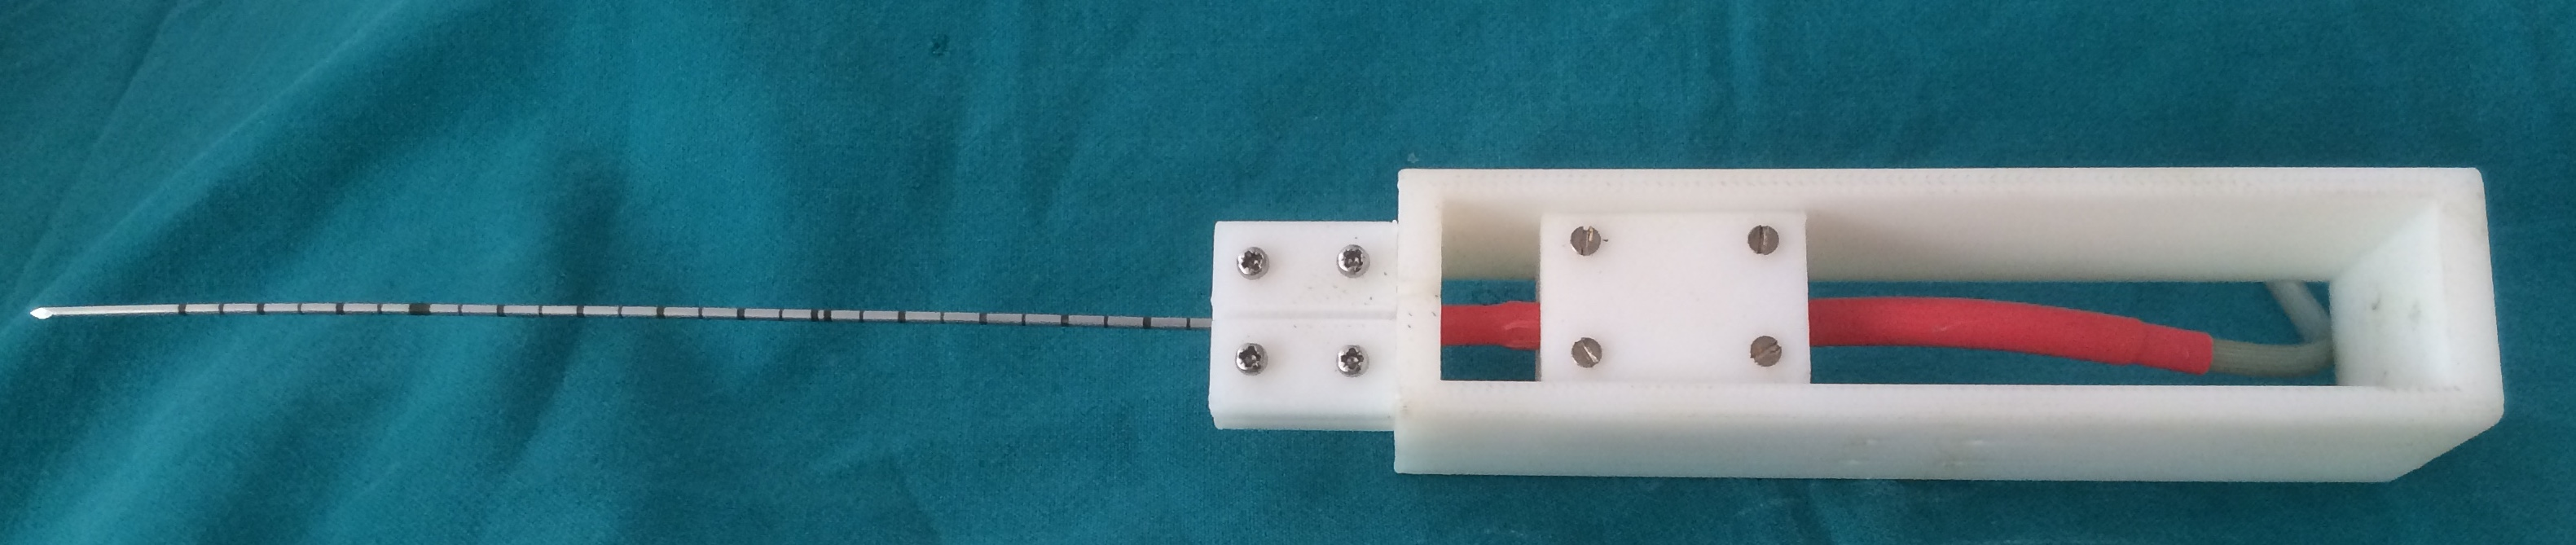
\includegraphics[width=\linewidth]{images/new_assembly.jpeg}
	\caption[The crioablation needle holder]{The crioablation needle holder}
	\label{fig:New_holder}
\end{figure}

\subsection{ATI Nano 17}
The ATI Nano 17 is the force sensor attached between the WAM tool flange and the needle holder.
It's a small six axis force/torque sensor with silicon strain gages.
The one available in Altair Laboratory has the SI-50-0.5 calibration whose sensing range and resolution has been reported in \tablename{ \ref{Nano_calib}}.
By supplying the transformation between the sensor and the needle tip, the software in its data acquisition \textit{NetBox} provides the measured wrenches correctly applied at the needle tip frame.

\begin{table} 
	\centering
	\begin{tabular}{lcc}
		\toprule
		& Sensing ranges  & Resolution\\
		\midrule
		$\mathrm{F_{x}}$& 50N & 1/80N\\
		$\mathrm{F_{y}}$& 50N & 1/80N\\
		$\mathrm{F_{z}}$& 70N & 1/80N\\
		\midrule
		$\mathrm{T_{x}}$& 500Nmm & 1/16Nmm\\
		$\mathrm{T_{y}}$& 500Nmm & 1/16Nmm\\
		$\mathrm{T_{z}}$& 70Nmm & 1/16Nmm\\
		\bottomrule
	\end{tabular}
	\caption[ATI Nano 17 calibration]{ATI Nano 17 SI-50-0.5 calibration data}
	\label{Nano_calib}
\end{table}

\section{Software Architecture}\label{GeneralArchitecture}
The teleoperation schema has been implemented on three machines: two Linux machine and a Windows machine.
The communication relays on the ROS framework and on a custom made socket.
The socket acts as a bridge between the ROS environment and the windows machine.
Two nodes that control the two manipulators, implementing respectively the master's and slave's Two-Layer controller, are connected through a couple of network simulator node.
In the middle a \textit{frame mapper} node maps the frame reference between the two manipulators.\\
The communication between the nodes relays on a custom ROS message which embeds all the information required both by the Two-Layer algorithm and the teleoperation strategy implemented at the transparency level.
The message structure is reported in \tablename{ \ref{message}} while the software architecture is sketched in \figurename{ \ref{sch:Harware_Arch}}.
Finally in \figurename{ \ref{sch:Teleop_topics_node}} we show an overview of the ROS nodes and topics involved. They will be explained within this section.
\begin{table}
\centering
\begin{tabular}{l l}
	\toprule
	\textbf{Message type} & \textbf{Name} \\ 
	\midrule
	std\_msgs/Header & header \\ 	
	geometry\_msgs/Pose & pose \\ 	
	geometry\_msgs/Twist & twist \\ 	
	geometry\_msgs/Wrench & wrench \\ 	
	std\_msgs/Float64 & energy\_request \\ 	
	std\_msgs/Float64 & power\_send \\ 
	\bottomrule
\end{tabular} 
\caption[The custom ROS message structure]{The custom ROS message structure}
\label{message}
\end{table}

\begin{figure}
	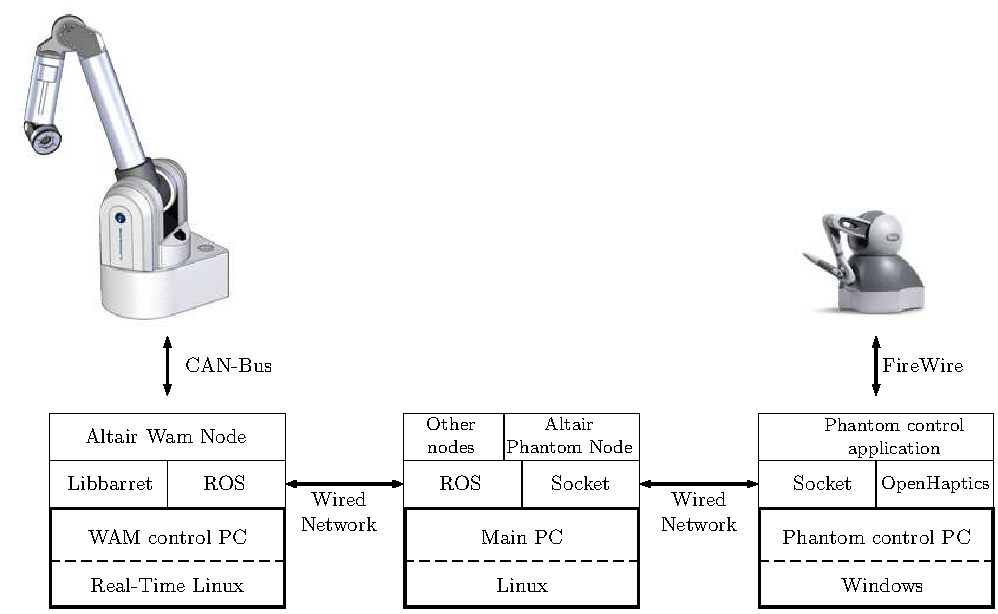
\includegraphics[width=\linewidth]{schemas/Hardware_Arch.pdf}
	\caption[Architecture overview]{Hardware/Software overview of the teleoperation architecture}
	\label{sch:Harware_Arch}
\end{figure}
\begin{figure}
	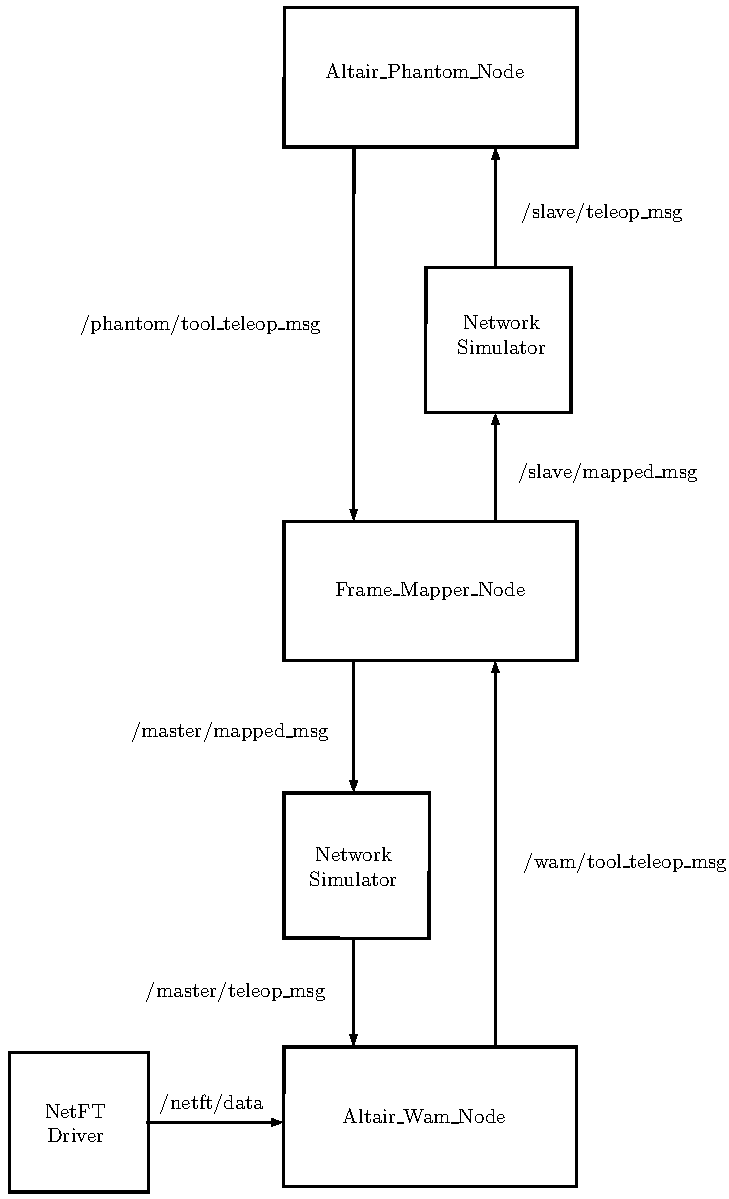
\includegraphics[height=\linewidth, angle =90]{schemas/Teleop_topics_node.pdf}
	\caption[ROS nodes and topics]{Nodes and topics in the implemented architecture }
	\label{sch:Teleop_topics_node}
\end{figure}
\subsection{ROS}
The Robot Operating System (ROS) \cite{ROS} is a open-source framework
based on the component-based software engineering paradigm that provides
the middleware for inter-process communication. Initially developed by the Stanford 
Artificial Intelligence Laboratory its development continued at Willow Garage, a robotics research institute, and now it's maintained and improved under the action of the ORSF foundation \cite{ROS}.

As a meta-operating system, ROS offers features such as hardware abstraction, low-level device
control, implementation of commonly used functionalities, message communication between processes and package management.
It uses an asyncronouse publish/subscribing mechanism  made possible by
message standardisation and incapsulation that make the external interface
of every node as general as possible, allowing quick nodes exchange and, thus,
great architectural flexibility.
Each indipendent block, called \textit{node}, executes a particular task of a process and can communicates with other nodes through \textit{topics}.
This allows to create complex architectures by aggregating many simpler entities and simplifies the use of different tasks  or different methods for the same task.

Additionally to the message-passing system, the core ROS component,
called \textit{roscore}, maintains a global execution time for the nodes to achieve
synchronisation. Each node executes separately with its own internal clock
driven by the set execution rate. At every message sent/received, containing
the internal time information, the core component updates the global time by
following the execution status provided by these messages.


\subsection{Frame Mapper}
The frame mapper node is fully transparent to the application and acts by matching both pose and force reference between the two manipulators.
To keep the developed architecture and each node inside it as general and modular as possible with the purpose of reusability of the developed master and slave nodes, we develop this node in a such a way it could match any pair of manipulators by providing, in its configuration, the transformation between the master and the slave base frame.\\
When launched, the node computes the difference between the two initial poses, then applies the proper transformation in both directions.\\
It could operate with any custom message type, the only requirements is the definition of a pose message inside the custom generated message.

\subsection{WAM control}\label{WAM_contol}
The WAM control node (\texttt{Altair\_Wam\_Node}) runs on the first machine, which execute the Ubuntu Linux 14.04.1 distribution patched with real time Xenomai co-Kernel.
This node is build on top of the Libbarret SDK. It continuously streams the status of the robot to the ROS infrastructure by publishing a set of topics with ROS standard messages.  It provides the following informations:
\begin{itemize}
	\item \textbf{End-effector position} referred both to the base and the tool frame of reference.
	\item\textbf{ End-effector twist}.
	\item \textbf{End-effector wrench}.
	\item \textbf{Joints position}.
\end{itemize}
It offers some convenient ROS services to exploit simple actions like autonomous reaching of a desired configuration or the ability of idleing the robot (means the robot is gravity compensated and free to move by hand).\\
On the basis of the ROS message received, the node engages the proper controller among the implemented ones.\\
This is possible by sending the control message to the proper control topic from the set of the topics the node subscribe itself.
There are eight controller available right now: Cartesian position, Cartesian orientation, Cartesian pose (which is the combination of the two previous ones), Cartesian velocity, Cartesian wrench, joint position, joint velocity and finally the Two-Layer controller developed for this work.\\
The Two-Layer controller provides the implementation of the passivity layer, as described in Section \ref{TwoLayer_improvements}, with the only difference that each threshold is designed as a range (a bottom and top thresholds) without violating the constraints between these variables, as explained in Section \ref{teleop_Ham-Port-with-Tank}.\\
The transparency level implements the control strategy. For this work it's a position PD controller, which is the same for the two teleoperation schemas tested and implemented.
It also provides the ability to filter the incoming control position, in order to smooth the control action when the input signal is noisy, as it happen with the measurements received from the Phantom Omni.
The output of the node, the passivated control torque in task space,  is passed to the underlying Libbarret real-time subsystem in charge of the low level control of the robot.

\subsection{Phantom Omni control}
Because of the lack of support for the modern Linux kernel, either for the old firewire model, and for the latest USB model, the Phantom Omni is physically attached and controlled on a Windows machine.
The interface with the ROS environment is ensured through a custom designed network socket connection.\\
The Phantom control node (\texttt{Altair_Phantom_Node}) runs on another Linux machine, and it could establish a bidirectional communication with the Windows machine up to 1kHz.
The design of the control node provides an abstraction of the Phantom manipulator in such a way that the socket interconnection could be easily replaced by a native device communication, through the OpenHaptics API, when the proper device driver will be available.
In fact on the Windows machine, the software simply receives commands from the remote controller and send back the Phantom status.

On top of this device abstraction, a general, abstract \textit{Phantom controller} has been designed. It's a partially implemented class which defines the standard \textit{Phantom controller} interface and implements a common thread that streams to the ROS network the device status in the same way the WAM control node does.
With this design, each specialization of the Phantom controller could be simply loaded into the Phantom ROS node and managed inside it in a standard way.
For this work, two specializations of the Phantom Controller have been written: one for the position-position architecture and one for the position-force architecture.
These specializations share the passivity layer implementation and most of the controller design with the WAM control node. 

\subsection{Network Simulator}
This node has the purpose to simulate a real network environment.\\
It could provide constant and time-varying delay with packet losses.
A couple of this node provides the communication delay in both direction.

\subsection{Neft node}
This node simply reads the wrench value from the ATI Nano 17 NetBox and streams it to the ROS network.

\subsection{Virtual visualizer}
The setup includes a virtual visualizer, based upon RVIZ, where a model of both the manipulators could be seen in a 3D environment.
This tool is useful for a pre-operative check on the correctness of the transformation applied to the commanded pose for each manipulator.

\begin{figure}
	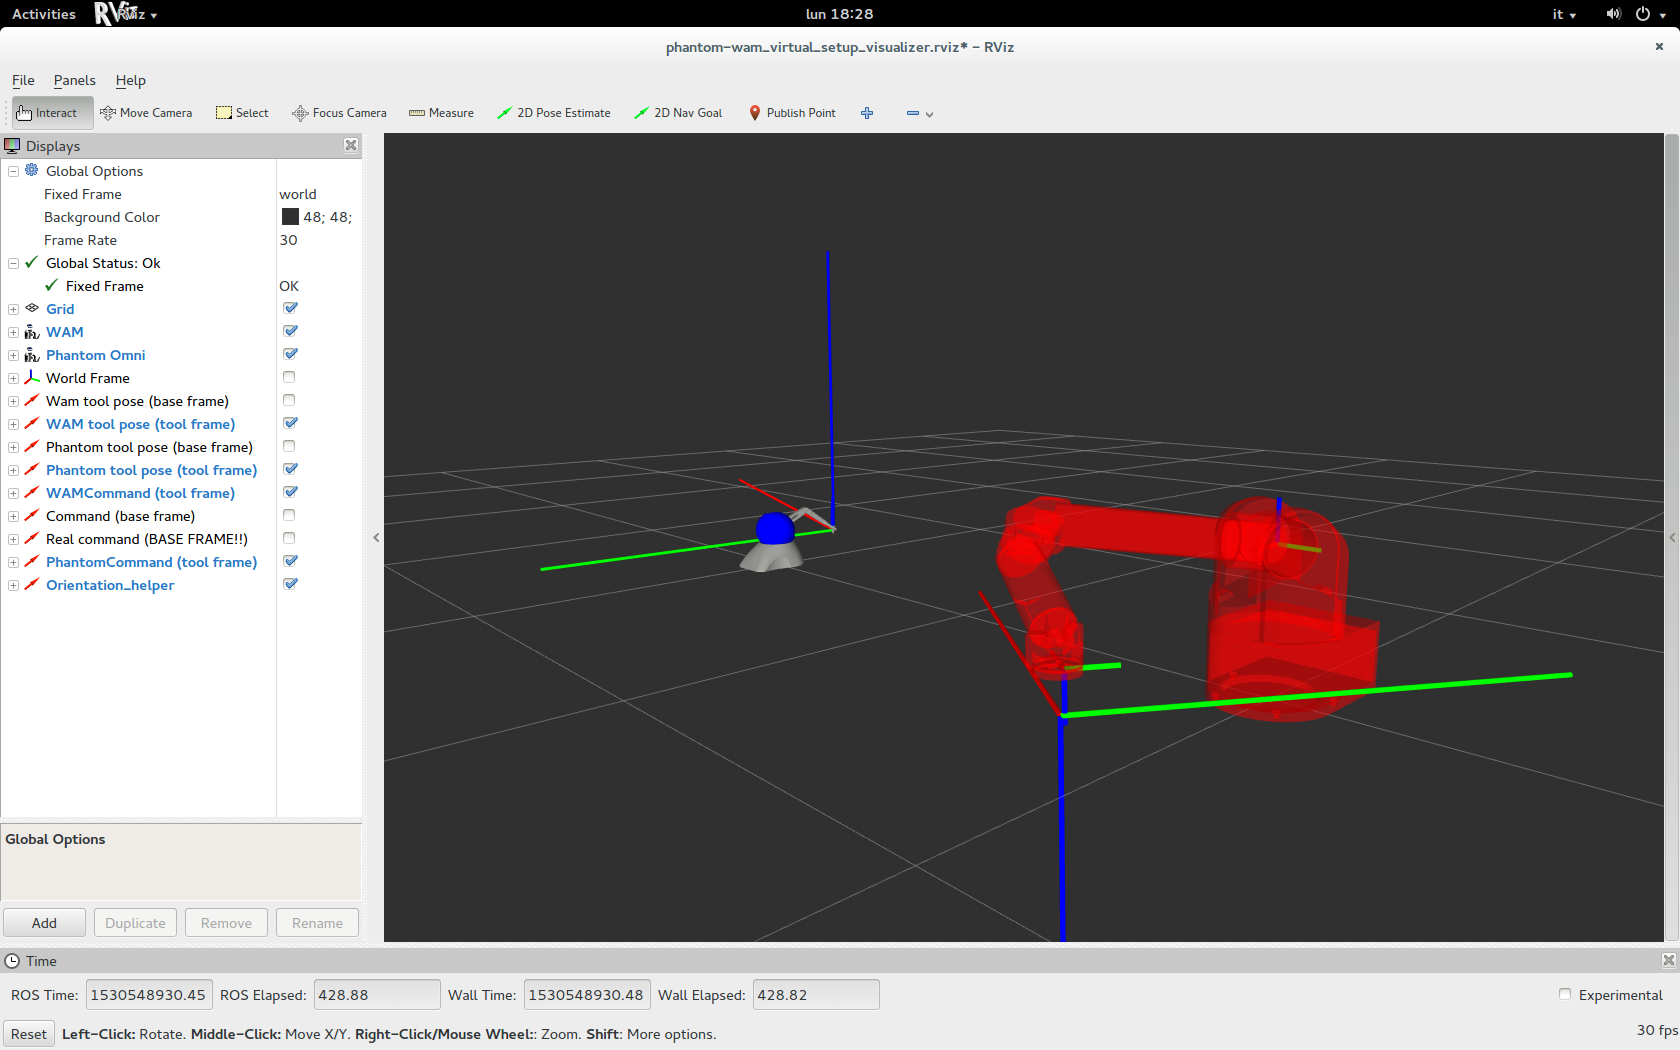
\includegraphics[width=\linewidth]{images/Visualizer.png}
	\caption[The visualizer]{Screenshot of the visualizer in action}
	\label{fig:Visualizer}
\end{figure}

\subsection{Setup limitations}
Because of the only tree translational degrees of freedom actuated on the Phantom Omni, this setup implements only a translational bilateral coupling.
This means that also the energy computation, both at master and slave sides, is performed only on translation.\\
The energy evaluated is the one flowing from the controller to the robot.
The lack of actuation means that no torque is exerted on the master and consequentially the instantaneous power is always equal to zero.\\
Because we cannot control the orientations, for them we have to relay on a unilateral teleoperation schema.\\
Unfortunately we cannot measure the real interaction force with the operator, but only the commanded one. However when the force on one axes exceeds the maximum values that the Phantom Omni could render, its APIs crops the value to 3.3N. This limits the transparency of the system so we set $K_{f}$ looking for a trade off to achieve a good transparency, meaning that the operator is still able to distinguish the insertion stage from the free motion.



%%%%%%%%%%%%%%%%%%%%%%5
\clearpage
\thispagestyle{empty}